While testing and analysing the 110V - 3kW LLC converter, I noticed that the maximum heat was generated in the transformer (with temperatures rising upto 80°C at maximum load)\\
I thought that, if we can redo the calculations for the transformer, making the design more efficient, we can reduce the heat generated in the transformer.\\
In the current version, we are using the EE55/28/21 core with N87 material for the transformer.\\
I did some research, and finally decided to use the PQ40/40 core with PC47 material for the transformer.
\subsection{Specifications of PQ40/40 Core}
From the \href{https://product.tdk.com/en/search/ferrite/ferrite/ferrite-core/info?part_no=PC47PQ40/40Z-12}{datasheet}, and \href{https://web.eecs.utk.edu/~dcostine/ECE482/Spring2014/materials/magnetics/MagneticsTables.pdf}{magnetics data}:
\begin{itemize}
    \item Effective Magnetic Path Length : $102 mm$
    \item Effective Cross-Sectional Area : $201 mm^2$
    \item Effective Core Volume : $20500 mm^3$
    \item AL Value: $4300 nH/turn^2$
    \item Core Window Area : $326 mm^2$
    \item MLT value = $83.9mm$
    \item Relative Permeability = $\mu_r = 2300$
    \item Dimensions: A1: 40.5 mm, A2: 28.0 mm, B: 37.0 mm, øC: 14.9 mm, 2D: 39.75 mm, E: 28.0 mm, 2H: 29.5 mm (Figure \ref*{fig:image3})
\end{itemize}
\begin{figure}[H]
    \centering
    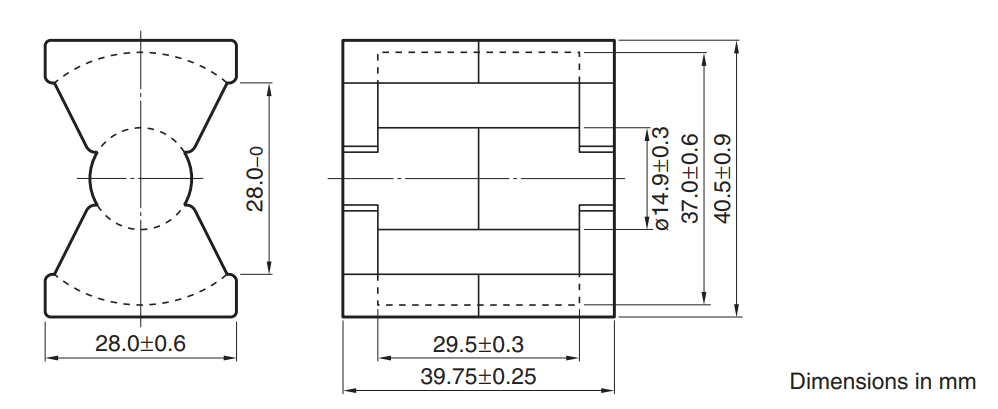
\includegraphics[width=0.8\textwidth]{images/image3.png}
    \caption{Cross-Section View of the PQ40/40 Core}
    \label{fig:image3}
\end{figure}

\subsection{Why PQ40/40 Core?}
\begin{itemize}
    \item \textbf{Power Handling Capability:} The PQ40/40 core has a large cross-sectional area ($2.01 cm^2$) and a substantial window area ($2.50 cm^2$), which allows it to handle higher power levels efficiently.
    \item \textbf{Magnetic Shielding:} PQ cores provide better magnetic shielding compared to other core shapes like EE or ETD cores. This helps in reducing electromagnetic interference (EMI) propagation, which is beneficial in high-frequency applications like our LLC converter.
    \item \textbf{Thermal Management:} The large core size of PQ40/40 allows for heat dissipation, which is important for maintaining thermal stability in air-cooled designs. This helps in managing the heat generated due to core and winding losses.
    \item \textbf{Mechanical Stability:} PQ cores are known for their mechanical stability and robustness, which is advantageous in applications where the transformer might be subjected to mechanical stress or vibrations.
\end{itemize}

\subsection{Material Selection: PC47 Ferrite}
\begin{itemize}
    \item \textbf{Low Core Losses:} PC47 material exhibits low core losses at high frequencies, which is essential for maintaining high efficiency in our LLC converter. At 100kHz and 200mT, the core loss is 250 kW/m³ at 100°C, which is lower compared to other materials like PC40 and PC44.
    \item \textbf{High Saturation Flux Density:} PC47 has a higher saturation flux density (530 mT at 25°C and 420 mT at 100°C) compared to other ferrite materials. This allows the core to operate at higher flux densities without saturating, which is beneficial for handling the power levels in our application.
    \item \textbf{Wide Frequency Range:} PC47 is optimized for a wide frequency range (10 kHz to 500 kHz), making it suitable for our LLC converter that operates at a resonant frequency of 127 kHz and can vary from 70 kHz to 300 kHz.
    \item \textbf{Thermal Stability:} PC47 material maintains its magnetic properties over a wide temperature range, with a Curie temperature above 230°C. This ensures stable performance even under varying thermal conditions, which is important for air-cooled designs.
    \item \textbf{Cost-Effectiveness:} While PC47 material offers superior performance, it is also cost-effective compared to other high-performance ferrite materials. This aligns with our requirement for an optimal design that balances performance and cost.
\end{itemize}
Taking into account the above-mentioned reasons, subsequent calculations for the following parameters were performed:
\begin{itemize}
    \item Primary Inductance ($L_p$) and number of turns at primary winding ($N_p$)
    \item Inductance at Secondary Winding and ($L_s$) and number of turns at secondary winding ($N_s$)
    \item Power Handling Capability of the Transformer
    \item Required Air Gap to get precise Inductance values.
    \item Wire cross section area for primary and secondary windings ($A_p$ and $A_s$)
    \item Litz Wire Calculations (For $\delta = 0.1mm, 300kHz$ the strand diameter was calculated to be 32AWG (0.2mm))
    \item Number of strands required for primary and secondary windings ($N_{strands,P}$ and $N_{strands,S}$)
    \item Winding lengths for primary and secondary windings ($L_P$ and $L_S$)
    \item Winding Volume for primary and secondary windings ($V_P$ and $V_S$)
    \item Winding Height Calculation
\end{itemize}
\noindent
The transformer design for the LLC converter using the PC47PQ40/40Z-12 core was expected to meet the specified requirements, with the calculated winding height being within the maximum winding height of 29.5 mm for the PC47PQ40/40Z-12 core, ensuring that the windings will fit within the core window area. The design considered the high-frequency operation, power rating, and the need for minimizing losses, providing a robust solution for the intended application.